%%%%%%%%%%%%%%%%%%%%%%%%%%%%%%%%%%%%%%%%%%%%%%%%%%%%%%%
%%%  Exploring the Semantic Context of News Events  %%%
%%%%%%%%%%%%%%%%%%%%%%%%%%%%%%%%%%%%%%%%%%%%%%%%%%%%%%%

\documentclass{llncs}

\newcommand{\superscript}[1]{\ensuremath{^{\textrm{#1}}}}

\usepackage{makeidx}  % allows for indexgeneration
\usepackage[hyphens]{url}
\usepackage{textcomp}
\usepackage{color}
\usepackage{listings}
\usepackage{multirow}
\usepackage{mathtools}
\usepackage{graphicx}
\usepackage{fancyvrb}
\usepackage{amsmath}
\usepackage{graphicx}
\usepackage[font=small,labelfont=bf]{caption}
\usepackage{pbox}
\usepackage{amsfonts}
\newcommand{\hg}[1]{\colorbox{yellow}{#1}}
\newcommand{\todo}[1]{\colorbox{red}{#1}}

\setcounter{MaxMatrixCols}{20}

% listing styles
\lstset{numbers=left, numberstyle=\tiny,basicstyle=\ttfamily\scriptsize, tabsize=2, keywordstyle=\underbar, stringstyle=\small, backgroundcolor=\color[gray]{0.94}, framexleftmargin=2pt}
\lstdefinestyle{rdfa}{numberblanklines=true, morekeywords={}}

%%%%%%%%%%%%%%%%%%%%%%%%
%%%  Begin Document  %%%
%%%%%%%%%%%%%%%%%%%%%%%%

\begin{document}

\frontmatter          % for the preliminaries
\pagestyle{headings}  % switches on printing of running heads
\mainmatter              % start of the contributions

%\title{Exploring the Semantic Context of News Events}
%\title{Spotting the Hidden Semantics of Newscasts}
\title{Generating Semantic Snapshots of Newscasts using Entity Expansion}
\author{Jos\'e Luis Redondo Garc\'ia\inst{2}, Michiel Hildebrand\inst{1}, Lilia Perez Romero\inst{1}, Giuseppe Rizzo\inst{2}, Rapha\"el Troncy\inst{2}}
\institute{EURECOM, Sophia Antipolis, France, \\
\email{\{redondo, giuseppe.rizzo, raphael.troncy\}@eurecom.fr}
\and
CWI, Amsterdam, The Netherlands, \\
\email{\{M.Hildebrand, L.Perez\}@cwi.nl}
}

\maketitle              % typeset the title of the contribution

%%%%%%%%%%%%%%%%%%
%%%  Abstract  %%%
%%%%%%%%%%%%%%%%%%

\begin{abstract}

% A recent trend in the newscasts domain consists on developing second screen applications that enable the user to further dive and improve his understanding of some particular news items, specially the complex word-scale controversial ones. The making of such applications requires the semantic annotation of the original newscasts as well as semantic enrichment for including background knowledge. Relying on video subtitles for providing time-based annotations of video content is a common method. However, it is insufficient to fully grasp the context of the newscasts being reported, simply because daily news reporting emphasizes on the last facts rather than on the narrative and causes of the reported event. In this paper, we propose a method that enables to search for and analyze related documents in order to generate semantic annotations that are closer to what viewers and experts in the domain expect to find while consuming newscasts. This approach generates annotations in the form of a ranked list of entities. We evaluate this method with respect to a gold standard made by domain experts for a set of BBC newscasts. Results of the experiments show the robustness in semantically annotating newscasts holding an Average Normalized Discounted Cumulative Gain of 66.4\%.

Generally newscasts in radio and television report about the latest event-related facts occurring in the world. \textit{Per se} a newscast delivers partial information thus neglecting the whole picture of the event that is often assumed as known. Relying exclusively on the broadcasted news item is therefore insufficient to fully grasp the context of the fact being reported. In this paper, we propose an approach to retrieve and analyze related documents in order to automatically generate semantic annotations, which provide viewers and experts of the domain with more comprehensive information to fully understand the news content. On the one hand, the approach takes as inputs the publication date and the newscast's title for gathering event-related documents on the Web, bringing more representativeness to the available knowledge. On the other hand, entities spotted in subtitles are merged with those found in related documents for further disclosing hidden relevant entities that were not explicitly mentioned in the original newscast. A ranking algorithm based on entity frequency, popularity peak analysis, and domain experts' rules sorts the annotations to generate the Semantic Snapshot of the considered Newscast (NSS). We benchmark this method against a gold standard generated by domain experts and assessed via user surveys for a set of BBC newscasts. Results of the experiments show the robustness of the approach holding an Average Normalized Discounted Cumulative Gain of 66.4\%.
%Lilia: not sure whether we can call our videos newscasts or whether they are more online news videos
\keywords{Semantic Video Annotation, Entity Expansion, Newscasts}
\end{abstract}

%%%%%%%%%%%%%%%%%%%%%%%%%
%%%  1. Introduction  %%%
%%%%%%%%%%%%%%%%%%%%%%%%%

\section{Introduction}
\label{sec:introduction}

With the emergence of both citizen-based and social media, traditional information television channels have to re-think their production and distribution workflow processes. We live in a globalized world, a vast playing field where events happening are the result of complex interactions between many diverse agents along time. Consumers require a huge effort to interpret those news mainly because of two issues: a) the \textit{need of background} problem: they probably need to be aware of other facts happened in a different temporal or geographical dimension, like one week ago or in a completely different region. And b), the \textit{need of completeness} problem: a single representation of an event is not enough to capture the whole picture, because it is normally incomplete, can be biased, or partially wrong. 

Recent gadgets and applications like second screen devices have recently irrupt as a good way of assisting the users in the challenge of becoming aware of that bigger picture of the event. In studies like \cite{Courtois2012} the authors tracked 260 tablet users, concluding that even there is only a modest uptake and interest in using secondary screens to digitally share opinions, the use of second screen interaction with television content is something the viewer qualitatively appreciate.

%\todo{GR: so far, you can find several textual data sources reporting on the same sets of news. Actually, you are likely to find more textual based sources than video}
%In addition, traditional text-based products are losing market share against other audiovisual solutions, in particular video. 
However even those applications offer a valid means, they still have to be fed with meaningful details concerning a newscast. The most common strategy to get this information is to go outside and analyze additional sources of information: today users have access to multiple news portals, different services for commenting and debating on the news, and social media that instantaneously spread news information. However this results in large amounts of unreliable and repeated information, leaving the user exploring on their own to try to build their version of a news event from large amounts of potentially related information and trying to find the truth in the middle of an ocean of rumors or hoaxes.

%\todo{GR: this is a jump -> from means (video, ...) to entities so why?}
Machine driven approaches have tried to alleviate the human difficulties when navigating this huge amount of information, but they struggle both in finding a good set of candidate documents and in properly analyzing them in order to offer relevant data back to the users. One strategy reported in literature for having such mechanisms implemented is to perform named entity extraction over the video transcript [REF?]. However, the set of entities obtained from such traditional operation is insufficient and incomplete for expressing the context of a news event  [REF]. Sometimes entities spotted over a particular document are not disambiguated because the textual clues surrounding the entity are not precise enough for the name entity extractor. While in other cases, they are simply not mentioned in the transcripts while being relevant for understanding the story. This is also an inherent problem in information retrieval tasks: a single description about the same resource does not necessarily summarize the whole picture. 
%\todo{GR: this is not true, or at least it depends on the domain/setting. It needs a pointer or just drop it.} 

%\todo{GR: what is this expansion thing? At this stage you are introducing to many things and it makes the introduction fragmented}
In this paper we present a novel approach for automatically retrieving and analyzing additional documents from the Web where the same event is also described. By increasing the size of set of documents to analyze, we increase the completeness of the context and the representativeness of the list of entities, reinforcing relevant entities and finding new ones that are potentially interesting inside the context of that news item. This approach, which we have called entity expansion is able to produce a ranked list of entities called  Semantic Snapshot Newscast (SSN) which expands the initial set of recognized entities with more relevant concepts that help to capture the whole context of the depicted event. The SSN can be later use to feed second screen applications assisting the viewer who watches the news, summarizing and generating quality snippets, or launch further  enrichment processes who bring related content the users could be also interested in watch. 

The paper is organized as follows: Section~\ref{sec:RelatedWork} presents the related works, Section~\ref{sec:ConceptExpansion} illustrates the approach depicted in this paper for generating SSN.
%, focusing in the collection of related documents, annotation of documents and entity filtering. 
Section~\ref{sec:Ranking} describes in depth the different ranking algorithms used for ordering the list of candidate entities generated in previous steps. Section~\ref{sec:Evaluation} explains the details of the ground truth, the measures considered in the evaluation, and the performance of our approach for different collection, filtering and ranking configurations, in order to see how better we are compared to the baseline and how close to the gold standard we can get. Finally Section~\ref{sec:Conclusion} summarizes the outcomes of the paper and describes our future work.

% State of the Art on Semantic annotation
%* State of the Art on Semantic annotation.
%Concerning the multimedia annotation the literature covers a wide range of different analysis techniques~\cite{ballan2011event}. One of the main approaches consists on running Named Entity Recognition (NER) over the textual information attached to particular video fragment. Those techniques are an essential component within the Information Extraction field that focus on: identifying atomic information units in texts, named entities; classifying entities into predefined categories (also called context types) and linking to real world objects using web identifiers (Named Entity Disambiguation). A growing number of APIs provide such a service, like AlchemyAPI\footnote{\fontsize{8pt}{1em}\selectfont \url{http://www.alchemyapi.com/}} or DBpedia Spotlight\footnote{\fontsize{8pt}{1em}\selectfont \url{http://spotlight.dbpedia.org/}}. 


%%%%%%%%%%%%%%%%%%%%%%%%%
%%%  2. Related Work  %%%
%%%%%%%%%%%%%%%%%%%%%%%%%

\section{Related Work}
\label{sec:RelatedWork}

%Studies on second screen applications and tools for supporting journalists. (WHY)
%\todo{GR:the first 4 lines are simply blabla and can be removed without loss}
%Television content in general and newscast in particular need the assistance of innovative applications which help the viewers and experts to get the most of them. One implementation design that has been deeply studied in the last years, mainly due to the increasing availability of tablets and tactile device is the "second screen application" paradigm. This kind of experiences open new possibilities for users watching television by complementing what is being displayed on the screen and offering a more active interaction with the content. 

%The need of a semantic snapshot.
The need of a semantic snapshot NSS for feeding certain applications and tools is already something we have experimented tin previous research works and prototypes like\cite{Redondo2014} which has revealed the great benefit for users of browsing the so called "context" of the newscasts. The same concept\footnote{\fontsize{8pt}{1em}\selectfont \url{https://vimeo.com/119107849}} has been presented to the forum Iberoamerican Biennial of Design (BID)\footnote{\fontsize{8pt}{1em}\selectfont \url{http://www.bid-dimad.org/}} with great reviews from the experts and scoring between the final 5 from a total of 200 candidates. At the same time, specialized researches like\cite{gynnild2014} highlight the importance in profesional journalism of algorithms, data, and social science methods for reporting and storytelling, under the term of computational exploration in journalism (CEJ). CEJ demands precise event descriptions for supporting the journalistic co-creation of quantitative news projects that transcend geographical, disciplinary, and linguistic boundaries.

%Entities in making sense (Semantic snapshot)  (WHAT)
All those news applications and tools need to be fed with the appropriate data to effectively assist viewers and professionals, and this information is normally broader than the one explicitly offered by the content itself. The hypothesis presented in this research paper states that this required knowledge can be represented in the form of a list of named entities called News Semantic Snapshot (SSN) which intends to describe the context of a newscast. This idea of using semantic annotations and named entities in particular is not new. In the context of the journalism activities, projects like NEWs have studied how to disambiguate named entity in the news domain by continuously learning while processing news streams\cite{Fernandez2012}. In the domain of Social Networks, entities are also used for identifying and modeling events and detecting breaking news. In \cite{Steiner2013} the authors emphasize the importance of spotting news entities in short user generated post in order to obtain a better understanding about what they are talking about. Entities have been also proven to be useful in producing good results in video classification when the textual information attached to a video contains temporal references (e.g. subtitles) Yunjia et al.~\cite{yunjia2013}. 

%How to create this semantic snapshot (Expansion idea) (HOW)
In order to build a comprehensive SSN the knowledge expressed in the newscast has to be extended with more information. Our approach performs a so called Entity Expansion process, which allows to collect on the fly additional documents in the Web describing the same event. 

\todo{GR: it starts here the related work}
In the literature there are already some approaches relying in similar expansion techniques, even if the final objetive is not spotting other event-related entities: instead, they pursue to pass from small number of named entities with the same type or category to a more complete named entity set. One of then is Google Sets\footnote{\url{http://googlesystem.blogspot.fr/2012/11/google-sets-still-available.html}}, an online service which is not longer available since 2014. Set expansion using the web is also closely related to the problem of unsupervised relation learning from the web\cite{Cafarella2005}, and set-expansion-like techniques have been used to derive features for concept-learning\cite{Cohen2000}, to construct ``pseudo-users'' for collaborative filtering\cite{Cohen99}, and to compute similarity between attribute values in autonomous databases\cite{Wolf2007}.

In 2007, RC.Wang and W.Cohen have been proposed their Set Expander for Any Language (SEAL) approach \cite{Wang2007}. SEAL works by automatically finding semi-structured web pages that contain lists of items and the aggregating these list in a way that the most promising items are ranked higher. SEAL is a language-independent system has shown good performance against previously published results like the already mentioned Google Sets. By using particular seeds and the top one hundred documents returned by Google, SEAL achieved 93\% in average precision in dataset from various languages. The same authors published an improved version of the algorithm one year later\cite{Wang2008} which increases the performance by handling unlimited number of supervised seeds. In each iteration, it expands a couple of randomly selected seeds while accumulating statistics from one iteration to another. Our approach does not rely in such kind of iterative mechanism, and focus more in maximize the quality of the search query for obtaining the most appropriate set of related documents to be analyzed.
 
Another approach in extending set of entities is \cite{Mai-Vu2010}, which combines the power of semantic relations between language terms like synonymy and hyponymy and grammar rules in order to find additional entities in the Web sharing the same category that the ones provides as input. Relying in Google they analyze documents for parsing semistructured text elements like tables and rank the final candidates using different ranking algorithms like PageRank. Several researchers propose a set expansion method using free text rather than semi-structured Web documents; for instance authors in \cite{Talukdar2006} presented a method for automatically selecting trigger words to mark the beginning of a pattern, which is then used for bootstrapping from free text. But still this approach looks for category related entities while in our case the driving force is more the event being shown in the news item.

Finally, a first implementation of the entity expansion algorithm was presented in\cite{RedondoGarcia2014}, including much less sophisticated document collection strategy, and considering only one ranking algorithm based on pure frequency. Even there is a first attempt in using DBpedia as a way to ensure the coherence of the final list of entities, there were no further efforts in use popularity measures or more elaborated rules for improve the accuracy of the results.

\hg{they are missing some examples of SSN and the related work made by Lilia}.


%%%%%%%%%%%%%%%%%%%%%%%%%%%%%%%%%%%%%%%%%%%%
%%%  3. News Concept Expansion Approach  %%%
%%%%%%%%%%%%%%%%%%%%%%%%%%%%%%%%%%%%%%%%%%%%
\section{News Concept Expansion Approach}
\label{sec:ConceptExpansion}
%In this section we present our algorithm to automatically generate News Semantic Snapshots out of a particular newscast. 
The approach we use to generate Newscast Semantic Snapshot is composed of the following stages: query formulation, document retrieval, semantic annotation, annotation filtering, and annotation ranking. Fig.~\ref{fig:namedEntityExpansion} depicts the process.

\todo{GR:names in Fig aren't consistent: either you use all lowercase of all uppercase}
\todo{GR:normalize the names in Fig with the ones reported in the paper}
\begin{figure}[h!]
\centering
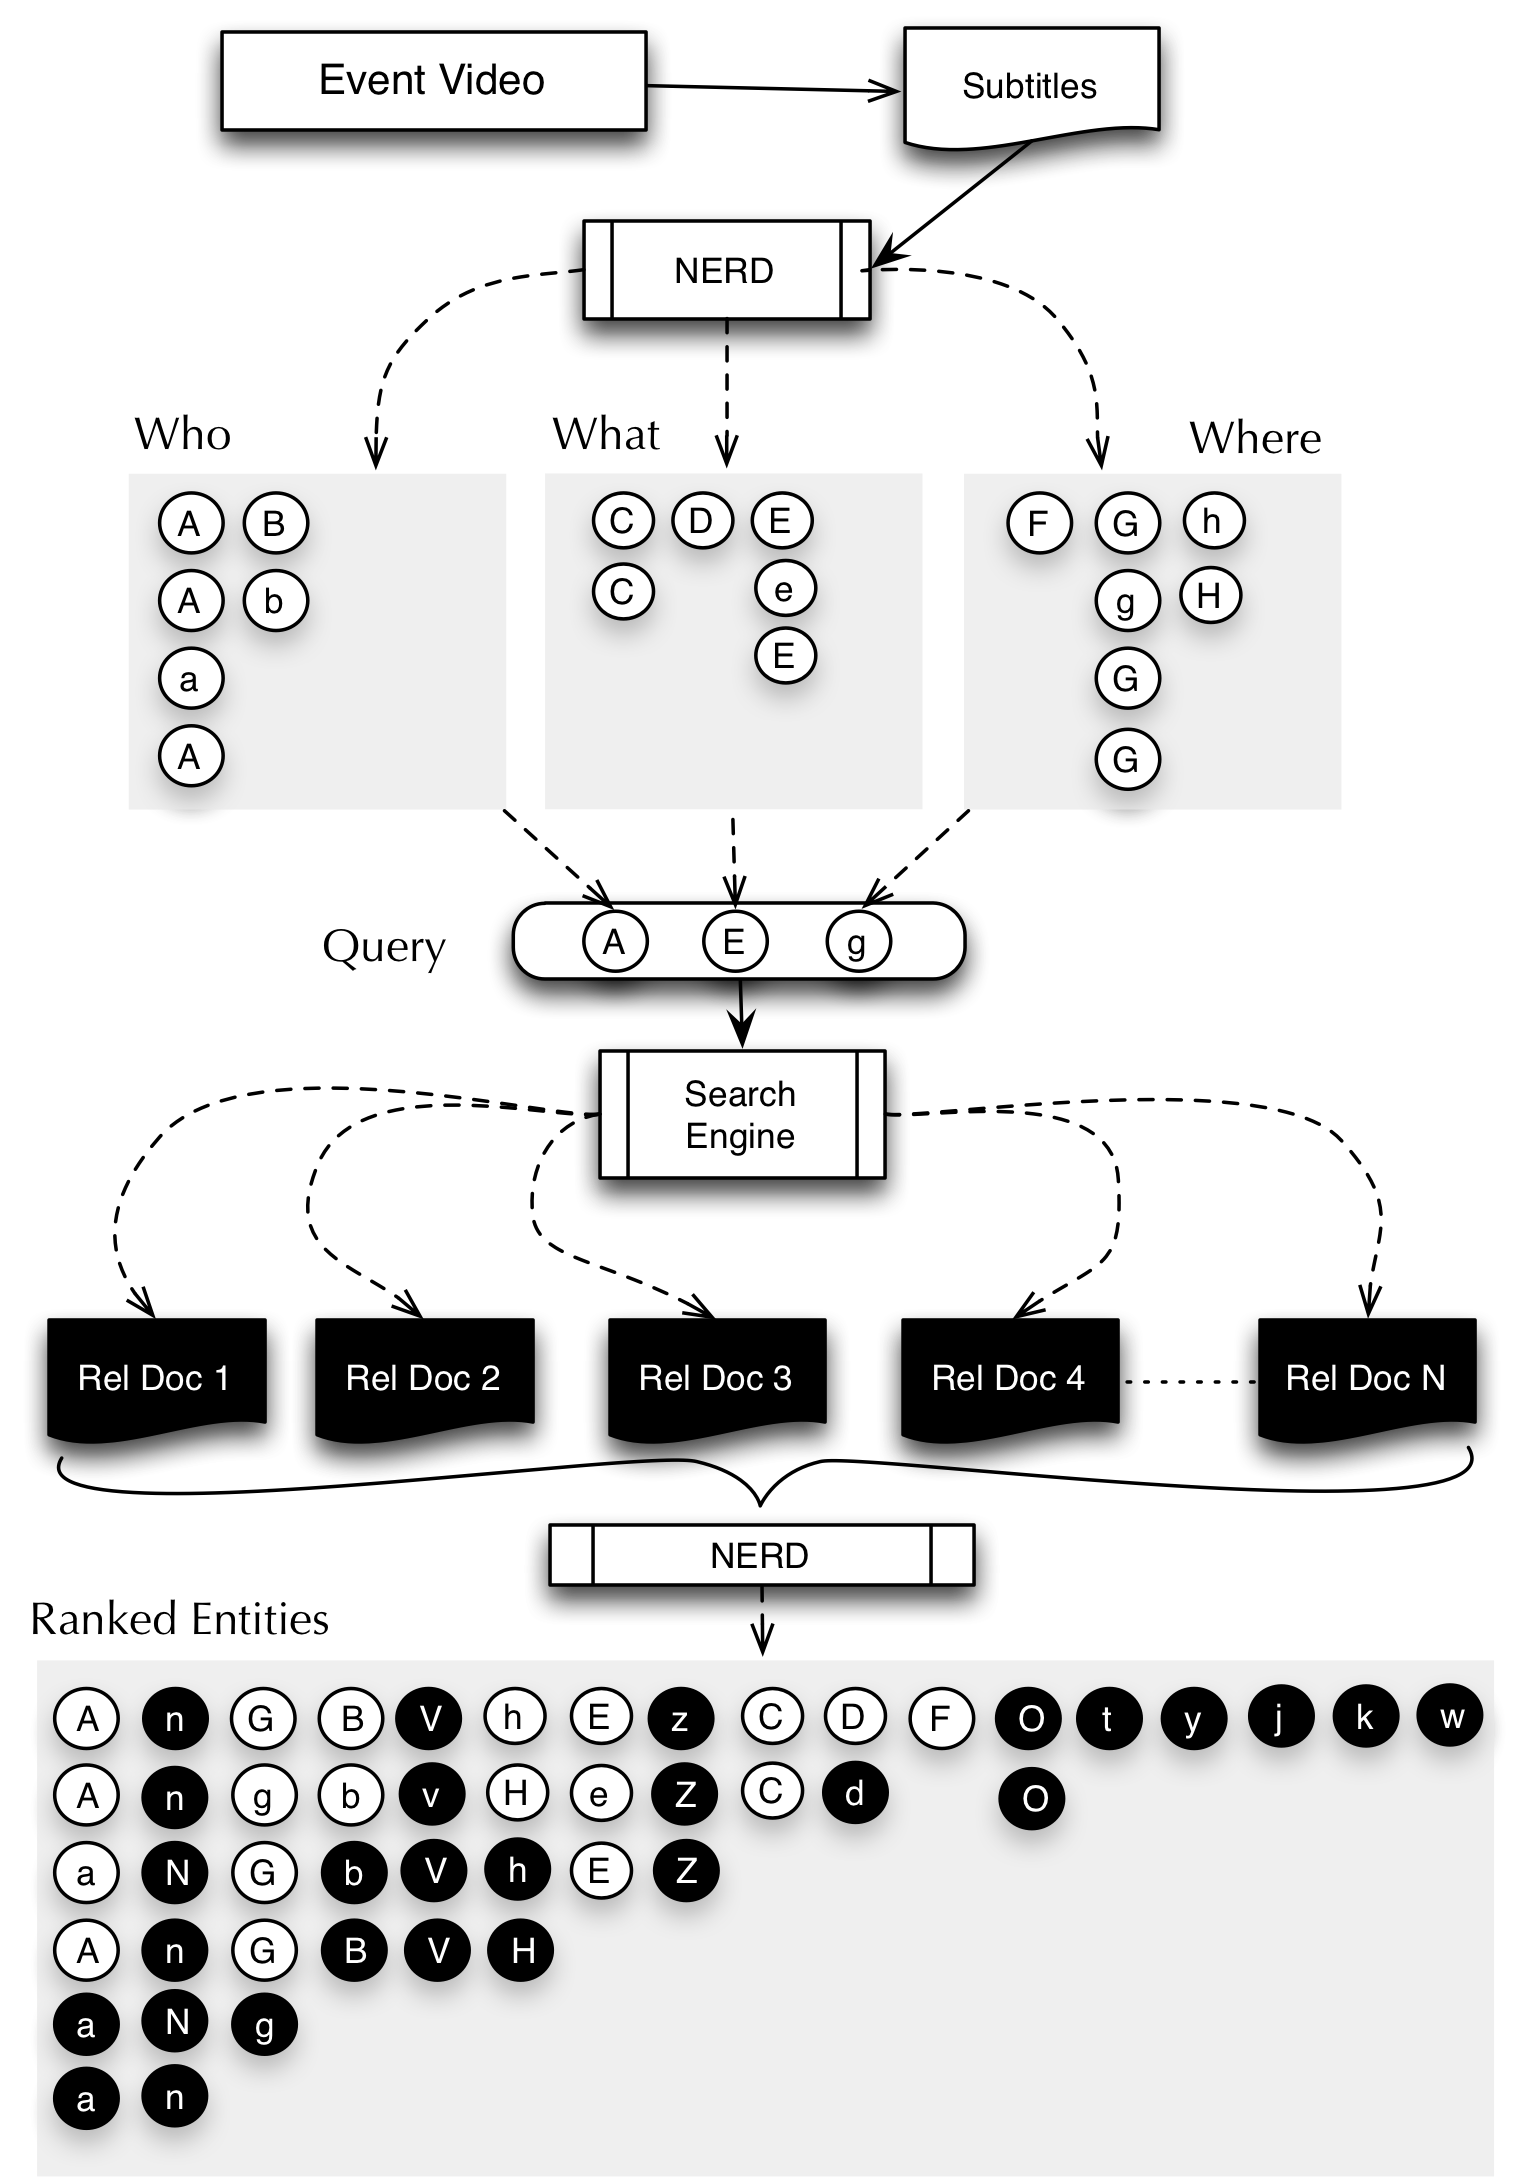
\includegraphics[width=1\textwidth]{figure/ExpansionDiagram}
\caption{Schema of Named Entity Expansion Algorithm.}
\label{fig:namedEntityExpansion}%\end{figure}
\end{figure}

{\bf Query Formulation} %OLD APPROACH
%The \emph{Five W's} is a popular concept of information gathering in journalistic reporting. It captures the main aspects of a story: who, when, what, where, and why~\cite{LiJia2007}. We try to represent the news item in terms of four of those five W's (who is involved in the event, where the event is taking place, what the event is about, and when it has happened) in order to generate a query that retrieves documents associated to the same event.
%First, the original entities are mapped to the NERD Core ontology, which considers 10 main classes: Thing, Amount, Animal, Event, Function, Organization, Location, Person, Product and Time. From those ten different categories, we generalize to three classes: the Who from \url{nerd:Person} and \url{nerd:Organization}, the Where from \url{nerd:Location}, and the What from the rest of NERD types after discarding \url{nerd:Time} and \url{nerd:Amount}.
Newscast broadcasters offer a certain amount of metadata about the items they publish, which is normally available together with the audiovisual content itself. In this work, we build the query $q= \left [ \text{h}, \text{t} \right ]$, where \textit{h} is the video heading, and \textit{t} is the publication date. The query is then used to as input of the retrieval stage.
%newscasts have with the following metadata: title, publication date, and the video transcript (non necessary timed). 
%We model a newscast as:
%\begin{equation}
%\text{q} =\left [ \text{t}, \text{d} \right ]
%\end{equation}
%Those different fields are taken from the video publisher and directly used as input for the rest of the expansion workflow without any pre-processing.

{\bf Document Retrieval}
The retrieval stage has the intent to collect event-related documents from the open Web. To some extents this process emulates what a viewer, who misses some details about the news he is watching, does: going to the Web, make a search, and get the most of the top ranked documents. Our programmatic approach emulates this human driven task by analyzing a much bigger set of related documents in a drastically smaller amount of time. The stage consists of retrieving documents that report on the same event discussed in the original video as result of the query \textit{q}. This phase in the expansion process has an key role in the upcoming semantic annotation stage, since it selects a set of the documents \textit{D} over which the semantic annotation process is performed. The quality and adequacy of the collected documents sets a theoretical limit on how good the process is done. 
%The more appropriate the collection of related document is, the better the final results will be.
%The different behavior of search engines make some alternatives more suitable than others for certain kinds of events. The way the resulting documents change in the search engines for a particular kind of event is a research question that will not be studied in this paper. 

{\bf Semantic Annotation} In this stage we perform a named entity recognition analysis with the objective of reducing the cardinality of the textual content from the set $D$ of documents $\{d_1, ..., d_n, d_{n+1}\}$ where $d_{i=1,..,n}$ defines the $i_{th}$ retrieved document, while $d_{n+1}$ refers to the original newscast transcript. Since most of the documents retrieved are Web pages, HTML tags and other annotations are removed, keeping only the main textual information. The feature space is then reduced and each document $d_i$ is represented by a bag of entities $E_{d_i}={e_{1_{d_i}}, ..., e_{n_{d_i}}}$, where each entity is defined as a triplet $(surface\_form, type, link)$. We perform a union of the obtained bags of named entities resulting in the bag of entities $E$ of the initial query $q$. 

{\bf Semantic Annotation Filtering and Clustering} The Document Retrieval stage expands the content niche of the newscast. At this stage we apply coarse-grained filtering of the annotations $E$ obtained from the previous stage, applying a $f\left ( E_{d_i}\right )\rightarrow  E'_{d_i}$ where $\left |E'_{d_i}  \right | < \left |E_{d_i}  \right |$. The filtering stategy grounds on the findings we obtained in the creation of the gold standard. In fact, when watching a newscast viewers better capture Person-type entities, as well as Organization-type and Location-type entities. The rest of less-specific and wider enclosed entities are more vague to be displayed on a television user interface and potentially less relevant for complementing the seed content. 
Named entities are then clustered applying a centroid-based clustering operation. As cluster centroid we consider the entity with the most frequent disambiguation $link$ that also have the most repeated $surface\_form$. As distance metric for comparing the instances, we applied strict string similarity over the $link$, and in case of mismatch, the Jaro-Winkler string distance~\cite{winkler2006overview} over the $surface\_form$. The output of this phase is a list of clusters containing different instances of the same entity.

{\bf Semantic Annotation Ranking}
%The different related documents collected and annotated in previous steps of the expansion algorithm contain the pieces of the puzzle that will allow to re-construct the big picture of the event. Unfortunately, those pieces come wrapped together with other less important parts which are not closely related with the event in particular and need to be put aside. By ranking the concepts, we make easier to (1) identify important entities from those which are, (2) group them in the top positions in order, (3) easy get rid of those which are not relevant to the considered event. The final NSS will be a subset of the top scored entities after the ranking algorithm.
The bag of named entities $E'_{d_i}$ is further processed to promote the named entities which are highly related to the underlined event. To accomplish such an objective, a we propose a ranking strategy based on entity appearance in documents, popularity peak analysis, and domain experts' rules sorts the annotations to generate the Semantic Snapshot of the considered Newscast (NSS).

%%%%%%%%%%%%%%%%%%%%%%%%%%%%
%%%  4. Ranking Strategy %%%
%%%%%%%%%%%%%%%%%%%%%%%%%%%%
\section{Ranking Strategy}
\label{sec:Ranking}
The unordered list entities is ranked to promote the entities that are potentially interesting for the viewer. The strategy we present in this work grounds on the assumption that the entities which appear often in the retrieved documents are important. We propose three different scoring functions for weighting the frequency of the entities. We then discuss two orthogonal functions which exploit the entity popularity in the time window considered for the event, and the domain experts' rules.
%and get rid of the long queue of less relevant concepts and noise generated by during the collection process. At the same time, this is also the most complicated task to perform: while computers are good in processing much large amounts of information and it would be possible to analyze hundreds of related documents, to decide which of the generated entities would be selected as relevant by a human is much more complicated. 

\subsection{Frequency-based Function}
The first intuitive way of ranking entities is according to their absolute frequency within the set of documents $D$. Let define $f_a(e_i, D)=[0,..,1]$, we define the score $S_F = \frac{ f_a(e_i, D) }{ |E| } $, where $|E|$ stands for the cardinality of all entities spotted across all documents. 
%Following this criteria, the more mentioned an entity is, the higher is will be scored. The opposite occurs to those barely mentioned all along the corpora, which will drop down in the final list of candidates. Therefore we have implemented a ranking strategy that orders entities according to their absolute frequency all over the collected documents: $S_{F}\left ( e \right ) =  f_{a}(e, D)$. 
%A second version of this simple strategy considers also confidence scores coming form the semantic annotation phase, in order to consider the certainty of the spotting process when detecting the entity $R_{score}\left ( e \right ) =  \sum_{1}^{i}c_{e_{i}}$ . 
In Fig.~\ref{fig:rankingStrategies} (a) we can observe how entities with lower absolute frequency are placed at the beginning of the distribution and discarded in the final ranking, where those with high $S_F$ are situated on the right side of the plot and they are elected to be part of the NSS.

\subsection{Gaussian-based Function}
Following a similar principle of the $S_F$, if an entity appears in a big number of documents, then it means the entity is relevant to be shown. However from the perspective of a television viewer, this is not always true: while it is true that entities appearing in just a few documents are probably irrelevant and not representative enough to be considered in the final results, entities spread all over the whole set of related documents are not necessary something the viewers would need to know about. In fact, they often represent entities that have been so present in media before that they have become too much obvious to the viewer. As consequence, we measure the Bernoulli appearance value of the entities across all documents as $f_{doc}(e_i)$, resulting in a Gaussian distribution where entities are condensed around the mean $\mu = \frac{|D|}{2}$ where $|D|$ is the cardinality of the retrieved documents (Fig.~\ref{fig:rankingStrategies} (b)). We have then approximated this behavior by using the function: $S_G = 1-\left | \frac{ f_{doc}(e_i) }{|D|} -1 \right |$.

\begin{figure}[h!]
\centering
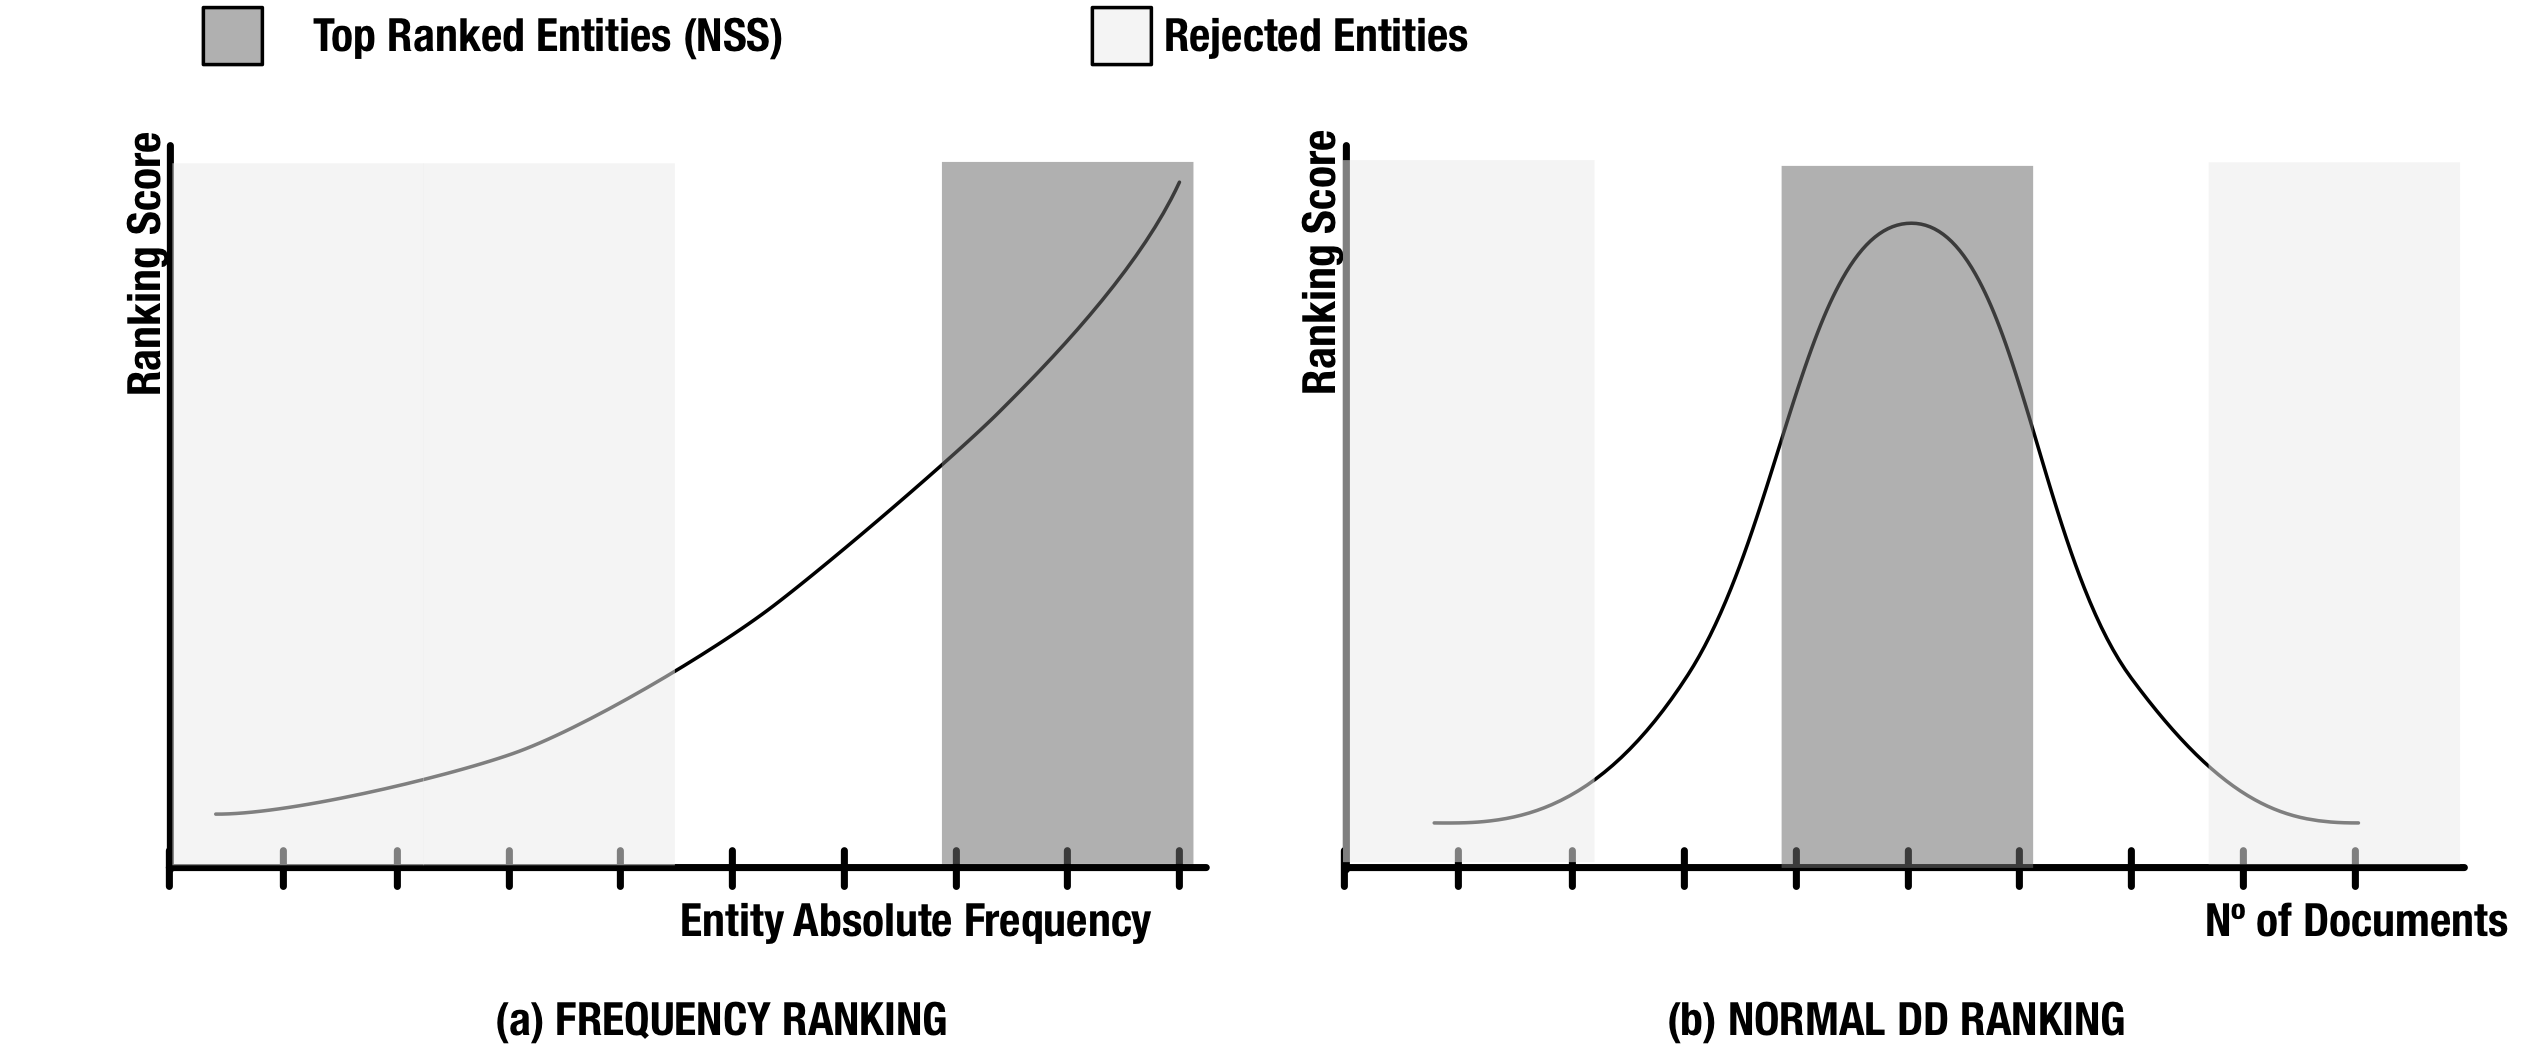
\includegraphics[width=0.9\textwidth]{figure/RankingStrategies}
\caption{(a) depicts the Decay function of the entity occurrences in the corpus, and the $S_F$ which underlines the importance of an entity being used several times in the corpus. (b) represents the Gaussian-based function $S_G$, with the entities highly impontant over the mean.}
\label{fig:rankingStrategies}%\end{figure}
\end{figure}

\hg{move to the experimental settings and Evaluation}
\subsection{TFIDF-based Function}
We measure the importance an entity in a document over a corpus of documents $D$ (reducing the absolute frequency of the entity) using the TF-IDF. This measure penalizes those entities appearing more frequently in general. The function is then as follows:

\begin{equation}
\begin{matrix}
tf(e_i,d_j) = 0.5 + \frac{0.5\times f_{a}(e_i,D)}{max\left \{ f_{a}(e_i',D) : e_i' \in d_j\right \}},   idf(e_i,d_j) = log\frac{\left | D \right |}{\left \{ d_j\in D  :  e_i\in d_j \right \}}
\end{matrix}
\end{equation}

However in our case the ranking algorithm has to be able to expose the importance of an entity inside the whole corpus $D$, while by definition TF-IDF refers only to the importance of an entity inside a particular document. 
For this reason we have extended this measure to capture the whole context of the newscast by aggregating the different $tf(e_i,d_j) \times idf(e_i,d_j)$ into a single function $tfidf^{*}(e_i,D)$ via the function $S_{TFIDF}= \frac{ \sum_{j=1}^{n} \sum_{i=1}^{n} tf(e_i,d_j) \times idf(e_i,d_j)} {|D|}$.
% Random Walks
% PageRank
% Use prior knowledge graph


\subsection{Popularity Function}
\todo{GR: separate the formalization part from the experimental settings, such as using GT, etc etc}
%Even the three ranking algorithms follow different considerations and principles, they end up exploiting the most precise an representative frequency values that the entity expansion process can provide compared to any other analysis over more reduced and probably partial newscast descriptions. 
We propose a weighting function based on a mechanism that detects variations in entity popularity values over a time window (commonly named as popularity peaks) around the date of the studied event. The functions proposed above exploit the frequency of the entities in documents as factor to measure its importance. However the frequency based approaches fail to explain the phenomenon of certain found entities which are barely mentioned in related document but suddenly become interesting for viewers. These changes are sometimes unpredictable so the only solution is to rely on external sources that can provide indications about the entity popularity. We then relied on Google Trends\footnote{\url{https://www.google.es/trends}}, which estimates how many times a search-term has been used in a given time-window.

\begin{figure}[h!]
\centering
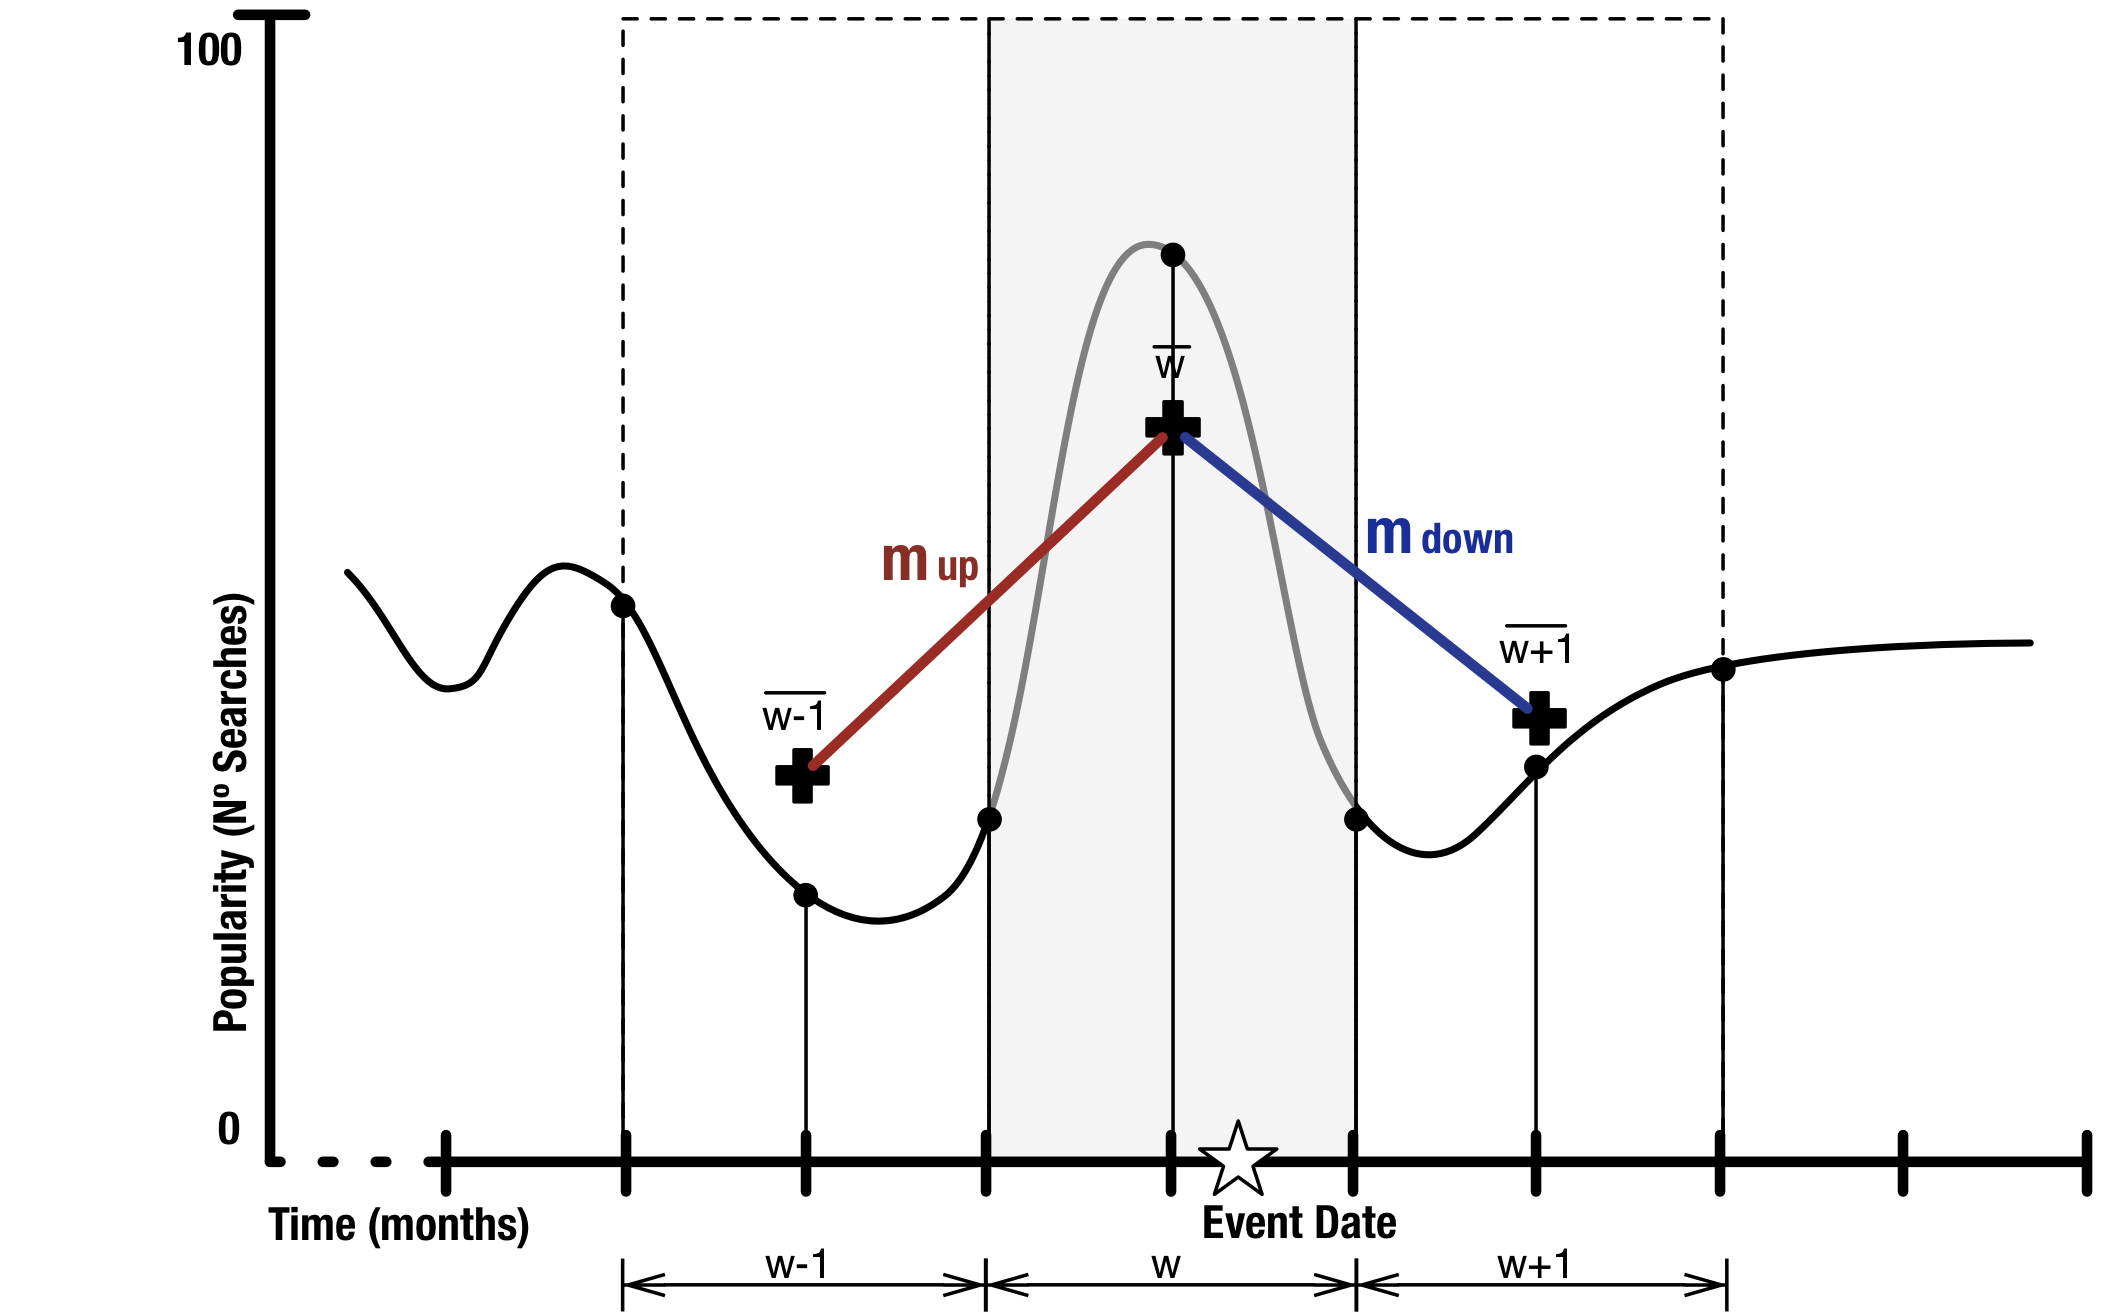
\includegraphics[width=0.7\textwidth]{figure/PopularityMeasure}
\caption{\todo{add proper caption}}
\label{fig:PopularityMeasure}%\end{figure}
\end{figure}

The procedure for getting $P_{peak}(e_i)$ is depicted in Fig.~\ref{fig:PopularityMeasure}. Using the label of an entity $e_i$, we obtain from Google Trends a list of pairs $[t, P]$ where $P\in[0,100]$ is the popularity score of an entity at the instant of time $t$. Afterward we create three consecutive and equally long temporal windows around $t$, the first one $w_{t}$ containing the date itself, another one just immediately behind $w_{t-1}$ and a last one after the previous two $w_{t+1}$. Given that Google Trends is giving results with a monthly temporal granularity, we have fixed the duration of such windows to 2 months in order to increase the representativity of the samples without compromising too much the validity of the selected values according with the time the event took place. 
In a next step we approximate the area inside the regions by calculating the average of the points contained in them, obtaining $\overline{w-1}$, $\overline{w}$ and $\overline{w+1}$. The slopes of the lines between $\overline{w-1}$ and $\overline{w}$, and $\overline{w}$ and $\overline{w+1}$ give the values $m_{up}$ and $m_{down}$ respectively, which are normalized and combined into a single score for measuring how significant the variation in volume of searches was for that studied entity label. When aggregating those two gradient, we scored $m_{up}$ higher in order to emphasize the irruption of a change more than the posterior distribution of the search term.
The last operation consists of merging the ranking produced by the pure strategies with the outcome from the popularity peaks detection algorithm. 
\todo{GR:better phrase this part. This is a pure approximation btw}
By studying the distribution of entities from to a particular newscast over their corresponding popularity scores, we have observed that it follows a Gaussian curve. 
\todo{GR:it needs to be adapted accordingly. We have now 3 S. Which on? And, isn't P something we should multiple}
With the aim of being selective enough and keep only those findings backed by strong evidence, we have filtered the entities with peak popularity value higher than $\mu+2*\sigma$ which approximately corresponds to a 2.5\%. Those entities will have their originally scores combined with the former ranking values via the the following equation: $S_{P}\left ( e \right )^{*} =  R_{score}\left ( e \right ) +Pop_{peak}(e)^{2} $.

\subsubsection{Expert Rules Function}
\todo{GR: dunno if it's propoer having this here, before the entire explaination. Most of the section should be moved later in the settings - supervised thing}
During the construction of the Ground Truth described in Section~\ref{sec:GoldStandard}, we have detected certain casuistic that can be materialized in rules that correct the scoring output produced by former ranking strategies. In particular, we have considered three rules to be applied over the three entity types considered in the ground truth, which have been deduced by comparing the average score per entity type in the gold standard $\overline{GT}_{typeScore}$ (see subsection~\label{sec:LessonsLearned})with the average score all over the entities.

- Organizations have the higher average score compared to the average, so they are eminently interesting for users.
- Persons have a fair average compare to the mean, so they should be somehow promoted as well.
- $GT_{Location}$ is quite low compared to the average so scores of entities from this type should be penalized.

In order to apply those rules over the previously generated rank, we multiply each entity by a factor that depends on the type of the entity according to the following equation: $R_{score}\left ( e \right )^{*} =  R_{score}\left ( e \right ) * (\overline{GT}_{typeScore} - \overline{GT}_{score})$.

A last rule also considered but independent of entity types is derived from one convention followed during the ground truth creation: each entity has to appear at least in two different sources in order to become a candidate. So all entities whose document frequency $F_{doc}(e)$ is lower than 2 are automatically discarded.

%%%%%%%%%%%%%%%%%%%%%%%%%
%%%  5. Gold Standard %%%
%%%%%%%%%%%%%%%%%%%%%%%%%
\section{Gold Standard}
\label{sec:GoldStandard}
We selected 5 short videos from the BBC One Minute World News website\footnote{\url{http://www.bbc.com/news/video_and_audio/}}. Each video lasted from 1 to 3 minutes. The selection covered a wide range of subjects specifically: politics, armed conflicts, environmental events, legal disputes, and social news. The intention behind this topic choice was to fit international audiences, since we planned to perform a user study with international participants. 

Subtitles of the videos were not available; therefore, a member of the team manually transcribed the speech in the videos.  After obtaining the transcriptions, the following steps were performed in order to obtain a set of unbiased candidate entities. We chose to focus only on entities of the types person, organisation and location because they can directly translate or answer three questions: Who is involved? What happened? Where did it take place? These questions are a subset taken from a well known concept in journalism known as the 5Ws (\textit{who}, \textit{what}, \textit {when}, \textit {where} and \textit {why}), which emphasizes the fundamental dimensions that an informative journalistic text should report on \cite{owenspencer}. Regarding the questions \textit{when} and \textit{why}, there where discarded because in order to acquire meaningfulness they need to be modeled not only by single entities but also by more complex relations between them that are out of the scope of the current paper.

\subsubsection{Subtitles}
All entities of the type person, organisation and location were manually extracted from each one of the video subtitles and added to the unfiltered list of entities (candidate set). 

\subsubsection{Image in the video}
The video image was visually analysed by a researcher and every time a recognisable person, organisation or location was portrayed this was also added as an entity to the candidate set. 

\subsubsection{Text in the video image}
The video was analysed for text appearing in the image. Whenever text appeared in the video image, for example in the form of nametag overlays, the named entities appearing in such tags were added to the candidate set. 

\subsubsection{Related entities }
In order to complement the candidate set with entities that might be interesting for the user, but are not necessarily found in the videos, we used the following two strategies:

\subsubsection{Suggestions of an expert}
We collaborated with a journalist with more than 6 years of experience as a writer/editor for important American newspapers and websites.  We configured an online survey to retrieve the expert’s feedback. In the survey we explained what named entities are and which types of named entities we needed. After this introduction we presented the videos to the expert. Following each one we asked him to list the named entities that, according to his criteria, would better serve the objective of showing interesting additional information to the users. The expert didn’t have access to the candidate set, and was completely free to suggest any named entity he wanted. 

\subsubsection{Related articles}
We used Google custom search to look for articles related to the video in three news sources: The Guardian, New York Times, and Al Jazeera online (English). We performed this search using the main terms in the videos’ title, for example, for ``Fugitive Edward Snowden applies for asylum in Russia'' we searched for  ``Edward''+``Snowden''+``asylum''+``Russia''. We limited the results to + - 3 days from the day when the video was published. We chose one document from each source, the one closest in topic and time to the video. We then extracted all named entities of the types person, organisation and location from the resulting documents. In order to keep the entities within a reasonable number for inclusion in a survey, we kept only the named entities that appeared in at least 2 related articles and dropped all the ones that only appeared in one.  The selected entities were added to the candidate set. 

\subsubsection{Refining the candidate set}
We refined the candidate set  comprised of all found entities by eliminating all duplicated named entities and standardising names. For example, when we had ``Barack Obama'' as an entity and ``Obama'' as another entity we eliminated the shorter one and left the complete name. 
	
A total of 99 entities were obtained from all videos. For a distribution of entities among types and videos please see Table \ref{table:entitydistribution}.

\begin{table}[h]
\begin{tabular}{| p{6cm} | l| l| l| l|}
  \hline
  \textbf{Video} & \textbf{Person} & \textbf{Organisation} &\textbf{Location} & \textbf{Total} \\
    \hline
  Fugitive Edward Snowden applies for asylum in Russia & 11 & 7 & 10 & 28 \\
    \hline
 Egypt's Morsi Vows to Stay in Power & 4 & 5 & 4 & 17 \\
    \hline
 Fukushima leak causes Japan concern & 7 & 5 & 5 & 13\\
    \hline
 Rallies in US after Zimmerman Verdict & 9 & 2 & 8 & 19 \\
    \hline
 Royal Baby Prince Named George & 15 & 1 & 6 & 22 \\
    \hline
    \textbf{Total}  & 46 & 20 & 33 & 99\\
  \hline
\end{tabular}
\caption[Table caption text]{Entity distribution in candidate set}
\label{table:entitydistribution}
\end{table}

\subsection{Online Survey}
We created an online survey with the aim of gathering information about the degree of interestingness of the entities in the candidate set. Based in \cite{vonBrzeski:2007:LCU:1321440.1321537} we define interestingness as to whether an entity is interesting, useful or compelling enough to tear the user away from the main thread of the document. 

Fifty international subjects participated in this online study. They responded an online call distributed via email and social networks. Their age range was between 25 and 54 years with an average age of 30.3 (standard deviation 7.3 years). 18 participants were female and 32 were male. Most of the participants were highly educated and 48 of them had either a university bachelor degree or a postgraduate degree. The main requisite for participation was that they were interested in the news and followed the news regularly, preferably through means that include newscasts.
During the interview participants were asked to choose at least 3 out of 5 videos according to their preferences. Then they were shown each one of the videos. After each video, they were asked to rate whether they would be interested in receiving more information about the named entities in the context of the news video and on a second screen or similar application. All the named entities from the candidate set related to the last seen video were shown in a list with ratio buttons arranged in a similar way to a three-point Likert-scale. The possible answers were ``Yes'' ``Maybe'' and ``No''. 

\subsection{Lessons learned from the online survey}
\label{sec:LessonsLearned}

The number of respondents per video were: ``Snowden'' 49, ``Morsi'' 34, ``Fukushima'' 42, ``Zimmerman'' 27, and ``Royal baby'' 15.

In order to calculate the interestingness scores from the users’ responses, we gave every answer a numerical value: ``Yes'' = 1, ``Maybe'' = 0 and ``No'' = -1.  We then obtained an average score for each entity using the number of participants that rated an entity and the score that each participant gave to that particular entity.  This average was used to obtain a ranking of all the entities in the candidate set according to user preferences. 

With the objective of finding out users preferences regarding the three analysed entity types: ``person '', ``organisation'' and ``location'', we calculated an average rating for each one of the entity types. The results in descending order were: organisation = -0,05, person = -0,24  and location = -0,52. These results clearly show a preference from users for the entities of the type organisation and person over those of the type location.


%%%%%%%%%%%%%%%%%%%%%%%%%%%%%%%%%%%%%%%%%%%%%%%%
%%%  6. Experimental Settings and Evaluation %%%
%%%%%%%%%%%%%%%%%%%%%%%%%%%%%%%%%%%%%%%%%%%%%%%%
\section{Experimental Settings and Evaluation}
\label{sec:Evaluation}
\todo{GR:main outcome in a few words, and then list the different points}

\subsection{Measures}
Measurements in terms of Recall and Precision, at 7 (average number of results selected as relevant by the users)
However those measures do not distinguish between differences in the rankings at positions 1 to p, which may be considered important for some tasks. For example, the two rankings in Figure 8.2 will be the same when measured using precision at 10.

This is why  the evaluation we will focus in the highly ranked relevant documents. Similar to Web search engines, we will apply an evaluation measure which will try to find as many relevant documents as possible, while still keeping the  premise that the top ranked documents are the most important. We will not perform measures in terms of efficiency. Even this kind of study is easier to quantify (most of the time it can be measured automatically with a timer instead of with costly relevance judgments) this falls outside the scope of this paper.
** How external items are measured.

Those are the key efficiency measurements we would like to perform,

** Mean average precision at 10  - single number summary, popular measure, pooled
relevance judgments.

** Average NDCG - single number summary for each rank level, emphasizes top ranked documents, relevance judgments only needed to a speciffc rank depth
(in our example 10).

** Recall-precision graph - conveys more information than a single number measure, pooled relevance judgments.

** Average precision at rank 10 - emphasizes top ranked documents, easy to understand, relevance judgments limited to top 10.

We will use the same same ranking algorithm on five different queries. We aim of an averaging technique is to summarize the effectiveness of a specific ranking algorithm across a collection of queries. Different queries will then have different numbers of relevant documents, as is the case in this example. Figure about recall-precision for the top ten rank positions.

Average between 5 queries.

SELECTING PRECISION AT N


\begin{figure}[h!]
\centering
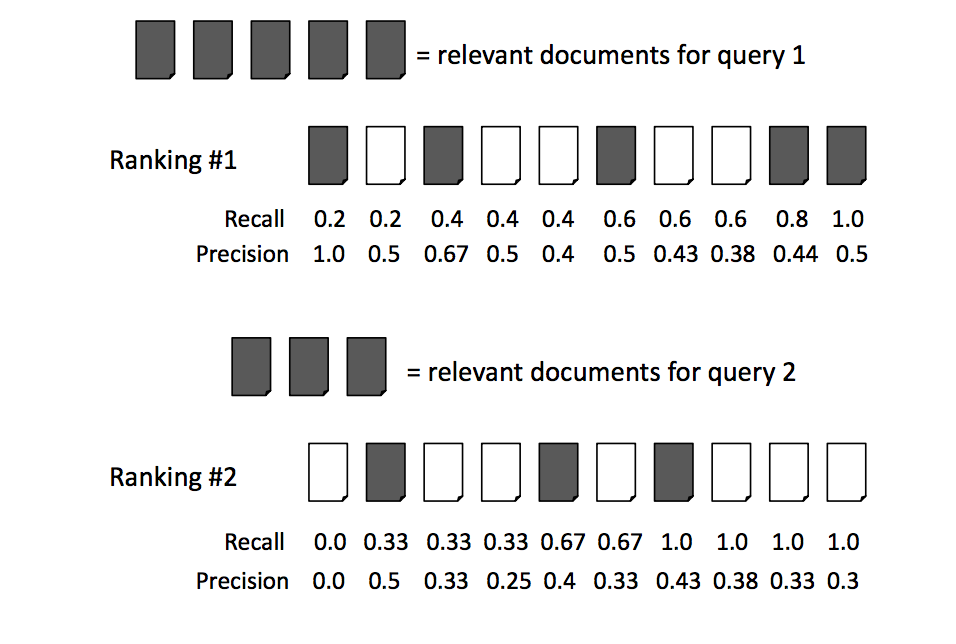
\includegraphics[width=0.9\textwidth]{figure/cumulativeGain}
\caption{Evaluation measures in document retrieval.}
\label{fig:namedCumulativeGain}%\end{figure}
\end{figure}

\subsection{Experimental Settings}
\label{sec:experimentalSettings}

\subsubsection{Document retrieval}
In this regard, we have relied on the Google Custom Search Engine API service\footnote{\fontsize{8pt}{1em}\selectfont  \url{https://www.google.com/cse/all}} by launching a query with the parameters specified in $\text{Query}_{Event}$. Apart of the query itself, the CSE engine considers other parameters that need to be tuned up. First, due to quota restrictions the maximum number of retrieved document is set to 50. As shown in the evaluation described in the Section~\ref{sec:evaluation}, this is enough for significantly extending the initial set of documents. But addition, we have also considered 3 different dimensions that could potentially influence the effectiveness in retrieving related documents:
\begin{enumerate}
 \item Web sites to be crawled. Google allows to specify a list of web domains and subdomains where documents can be retrieved from. This reduces the scope of the search task and, depending on the characteristics of the considered sources, influence the nature of the retrieved items: from big online newspapers to user generated content. At the same time, Google allows to prioritize searching over those whitelists while still considering the  whole indexed Web. Based on this, in our study we considered five possible values for this parameter:
a) AllGoogle: search over the whole set of Web pages indexed by Google.
 \begin{itemize}
  \item Newspaper whitelist. A set of 10 internationals English speaking newspapers chosen from \footnote{\fontsize{8pt}{1em}\selectfont  \url{http://en.wikipedia.org/wiki/List_of_newspapers_in_the_world_by_circulation}}
  \item Lilia's whitelist. A set of 3 international newspapers used in [Lilia] while building the ground truth used in Section~\ref{sec:evaluation}.
  \item Newspaper whiteList + Google. Prioritize content in Newspaper whitelist but still consider other sites.
  \item Lilia's whitelist + AllGoogle: Prioritize content in Lilia's whitelist but still consider other sites.
 \end{itemize}
 \item Temporal dimension. This variable allows to filter those documents which are not temporarily close from the day where the newscast was published. Assuming that the news item is fresh enough, this date of publication will also be fairly close to the day the event  took place. Taking $\text{PublishingDate}$ as a reference and increasing the window in a certain amount of days $d$,  we end up having $Time_{Window}=\left [ \text{PublishingDate}-d, \text{PublishingDate}+d \right ]$ The reason why we expand the original event period is because documents concerning a news event are not always published during the time of the action is taking place but some hours or days after or before. The final $Time_{Window}$ could vary according to many factors such as the nature of the event itself (whether it is a brief appearance in a media, or part of a longer story with more repercussion) or the kind of documents the search engine is indexing (from very deep and elaborated documents that need time to be published, to short post quickly generated by users). In this study we have considered two possible values for it: 2 weeks and one week temporal windows.
 \item In addition, Google Custom Search Engine makes possible to filter result according to the Schema.org types: 2 values:. Based on the study.
[NoFilter(Default), Person\&OrganizationFiltered]
\end{enumerate}

TABLE OF RESULTS
That makes $5 * 2 * 2 = 20$ different runs 

that we will study in the Section~\ref{sec:evaluation} in order to discover which configuration optimizes the expansion algorithm.

* Explain insights obtained from the survey. \% of entities coming from subtitles, form other sources, etc

\subsubsection{Entity Filtering}
\label{sec:settingsFiltering}

After some first trials it became evident that those many non-pure Named Entities which were not well considered by viewers and expert during the ground truth creation [Lilia] were dramatically dropping the scores for most of the considered ranking strategies. We have foreseen three different filtering approaches for getting rid of those undesired concept annotations:

\begin{enumerate}
\item Filter by type (F1). Filter annotations according to their NERD type. In our case, only \textbf{nerd:Person}, \textbf{nerd:Location}, and \textbf{nerd:Organization} entities.
\item Filter by confidence (F2). Second strategy consist on getting ride of entities with confidence score under first quarter of the distribution.
\item Filter instances (F3). Intuitively, people seems to be more attracted by proper names. Those names are normally uppercased. This filter keeps only concepts matching this rule.
\end{enumerate}

We executed different runs by applying those filters over the original annotations and their corresponding combinations, manly: (F1 - F2 - F3 - F1\_F2 - F1\_F3 - F2\_F3 - F1\_F2\_F3 ), resulting in significant improvement in the final scores as shown in Section~\ref{sec:FilteringExperiments}, in terms of different measures like Precision, recall, average precision, and NDCG.

\subsubsection{Entity Ranking}
\label{sec:settingsRanking}

All strategies considered, with and without Expert rules, with / without popularity.

\subsection{Results}


TABLE showing content. Measures

1) The problem with non strict Named Entities being promoted in TFIDF strategy is clearly alleviated for all filters and combinations. TF strategy has generally improved as well, but in a lower scale.
2) The TF strategy performs better than the current implementation of TFIDF in ALL cases.
3) Best Filter for TF strategy is F3 (0.523665971)
4) Best Filter for TFIDF strategy is the combination F1\_F3
5) I combined the results for both strategies via a) simple multiplication and b) their average value, see rows 4th and 5th. In both cases, the combination F1\_F3 seems to perform the best.


%%%%%%%%%%%%%%%%%%%%%%%
%%%  5. Conclusion  %%%
%%%%%%%%%%%%%%%%%%%%%%%

\section{Conclusion}
\label{sec:Conclusion}
We presented an approach for context-aware annotating news events, designed to precisely harvest program descriptions starting from named entities recognized in TV video transcripts. Because the entities initially spotted are typically insufficient for covering the broader range of concepts that best describe a particular news clip, we expanded this set by analyzing additional textual documents about the same event.

The evaluation indicates that we can successfully expand the initial set of recognized entities with more relevant concepts not detected by pure named entity recognition approaches and produce a more accurate ranking of important concepts that brings forward entities which user are more interested about.

Future: tailor ranking to particular types of news: sport, politics, regional, international, opinion, etc. Survey on 15 videos from the BBC about international facts. Evaluated over people in different countries.
semantic annotation for doing: summarizing topics/entities


%%%%%%%%%%%%%%%%%%%%%%%%%
%%%  Acknowledgments  %%%
%%%%%%%%%%%%%%%%%%%%%%%%%

\section*{Acknowledgments}
This work was partially supported by the European Union's 7th Framework Programme via the project LinkedTV (GA 287911).

%%%%%%%%%%%%%%%%%%%%%%
%%%  Bibliography  %%%
%%%%%%%%%%%%%%%%%%%%%%
\todo{many references are not compiled}
\bibliographystyle{abbrv}
\bibliography{NewsConceptExpansion}

\end{document}
